\documentclass[a4paper,12pt]{article}
\usepackage[utf8]{inputenc}
\usepackage{graphicx}
\usepackage{float}
\usepackage[spanish]{babel}
\usepackage{listings}
\usepackage{xcolor}
\usepackage{courier}
\usepackage[T1]{fontenc}

\definecolor{gris}{RGB}{123, 126, 132}
\definecolor{morado}{RGB}{81, 40, 155}
\definecolor{amarillo}{RGB}{253,151,31}
\definecolor{magenta}{RGB}{249,38,114}

\renewcommand{\lstlistingname}{Archivo}

\lstdefinestyle{customJava}{
    frame=tb,
    language=Java,
    backgroundcolor=\color{white},   
    commentstyle=\itshape\color{gris},
    keywordstyle=\bfseries\color{magenta},
    numberstyle=\color{morado},
    stringstyle=\color{amarillo},
    identifierstyle=\color{black},
    basicstyle=\footnotesize,
    breakatwhitespace=false,         
    breaklines=true,                 
    captionpos=b,
    keepspaces=true,                 
    numbers=left,                    
    numbersep=5pt,                  
    showspaces=false,                
    showstringspaces=false,
    showtabs=false,                  
    tabsize=2,
}

%opening
\title{Ejercicio No. 2. Carrera-Alumno (Consola)}
\author{Barrera Pérez Carlos Tonatihu \\ Profesor: José Asunción Enríquez 
Zárate \\ Web Application Development \\ Grupo: 3CM9 }

\begin{document}

\maketitle

\newpage
\tableofcontents
\newpage
\section{Introducción}
Este ejercicio tuvo como objetivo desarrollar un pequeño CRUD para la base de 
datos que se muestra en la figura \ref{fig:bd}.

\begin{figure}[H]
\begin{center}
 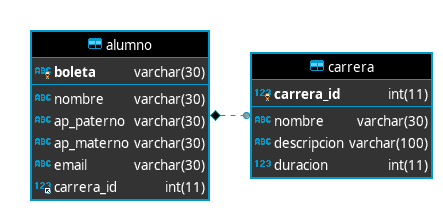
\includegraphics[width=\textwidth]{diagrama.png}
 \caption{Base de datos que se trabajo en MySQL}
 \label{fig:bd}
\end{center}
\end{figure}

Se utilizo el patrón DAO para realizar una implementación más limpia y que 
pudiera ser utilizada en un futuro.

\section{Desarrollo}

\subsection{Código}
\begin{lstlisting}[language=Java, style=customJava, 
caption={Alumno.java},captionpos=b,basicstyle=\fontfamily{cmss}\small]
package instituto;

import java.io.Serializable;

/**
 *
 * @author tonatihu
 */
public class Alumno implements Serializable {
    private String noBoleta;
    private String nombre;
    private String apPaterno;
    private String apMaterno;
    private String email;
    private Carrera carrera;

    public Alumno() {
    }

    public String getNoBoleta() {
        return noBoleta;
    }

    public void setNoBoleta(String noBoleta) {
        this.noBoleta = noBoleta;
    }

    public String getNombre() {
        return nombre;
    }

    public void setNombre(String nombre) {
        this.nombre = nombre;
    }

    public String getApPaterno() {
        return apPaterno;
    }

    public void setApPaterno(String apPaterno) {
        this.apPaterno = apPaterno;
    }

    public String getApMaterno() {
        return apMaterno;
    }

    public void setApMaterno(String apMaterno) {
        this.apMaterno = apMaterno;
    }

    public String getEmail() {
        return email;
    }

    public void setEmail(String email) {
        this.email = email;
    }

    public Carrera getCarrera() {
        return carrera;
    }

    public void setCarrera(Carrera carrera) {
        this.carrera = carrera;
    }

    @Override
    public String toString() {
        return "dto.Alumno{" + "noBoleta=" + noBoleta + ", nombre='" + nombre 
                + '\'' + ", apPaterno" + "='" + apPaterno + '\'' 
                + ", apMaterno='" + apMaterno + '\'' + ", email='" 
                + email + '\'' + ", carrera=" + carrera + '}';
    }
}
\end{lstlisting}

\begin{lstlisting}[language=Java, style=customJava, 
caption={Carrera.java},captionpos=b,basicstyle=\fontfamily{cmss}\small]
package instituto;

import java.io.Serializable;

/**
 *
 * @author tonatihu
 */
public class Carrera implements Serializable {
    private int id;
    private String nombre;
    private String descripcion;
    private int duracion;

    public Carrera() {
    }

    public int getId() {
        return id;
    }

    public void setId(int id) {
        this.id = id;
    }

    public String getNombre() {
        return nombre;
    }

    public void setNombre(String nombre) {
        this.nombre = nombre;
    }

    public String getDescripcion() {
        return descripcion;
    }

    public void setDescripcion(String descripcion) {
        this.descripcion = descripcion;
    }

    public int getDuracion() {
        return duracion;
    }

    public void setDuracion(int duracion) {
        this.duracion = duracion;
    }

    @Override
    public String toString() {
        return "dto.Carrera{id=" + id + ", nombre='" + nombre + '\'' 
                + ", descripcion='" + descripcion + '\'' + ", duracion=" 
                + duracion + '}';
    }
}

\end{lstlisting}

\begin{lstlisting}[language=Java, style=customJava, 
caption={GenericDAO.java},captionpos=b,basicstyle=\fontfamily{cmss}\small]
package instituto;

import java.sql.SQLException;
import java.util.List;

/**
 *
 * @author tonatihu
 * Created on 01-Jun-2019
 */
public abstract class GenericDAO <T>{
    public abstract void create(T entity) throws SQLException;
    public abstract void update(T entity) throws SQLException;
    public abstract T read(T entity) throws SQLException;
    public abstract void delete(T entity) throws SQLException;
    public abstract List<T> readAll() throws SQLException;

}
\end{lstlisting}

\begin{lstlisting}[language=Java, style=customJava, 
caption={CarreraDAO.java},captionpos=b,basicstyle=\fontfamily{cmss}\small]
package instituto;

import java.sql.PreparedStatement;
import java.sql.ResultSet;
import java.sql.SQLException;
import java.util.ArrayList;
import java.util.List;

/**
 * @author tonatihu
 * Created on 1/30/19
 */
public class CarreraDAO extends GenericDAO<Carrera>{
    private static final String SQL_INSERT = "insert into carrera(nombre, "
            + "descripcion, duracion) values (?, ?, ?)";
    private static final String SQL_UPDATE = "update carrera set nombre=?, "
            + "descripcion=?, duracion=? where carrera_id=?";
    private static final String SQL_SELECT = "select * from carrera "
            + "where carrera_id=?";
    private static final String SQL_SELECT_ALL = "select * from carrera";
    private static final String SQL_DELETE = "delete from carrera "
            + "where carrera_id=?";

    private final Conexion conexion;

    public CarreraDAO() {
        conexion = new Conexion();
    }

    @Override
    public void create(Carrera c) throws SQLException  {
        PreparedStatement ps = null;
        conexion.conectar();
        try {
            ps = conexion.createPreparedStatement(SQL_INSERT);
            ps.setString(1, c.getNombre());
            ps.setString(2, c.getDescripcion());
            ps.setInt(3, c.getDuracion());
            ps.executeUpdate();
        } finally {
            conexion.cerrar(ps);
            conexion.cerrar();
        }
    }

    @Override
    public Carrera read(Carrera c) throws SQLException  {
        PreparedStatement ps = null;
        ResultSet rs = null;
        conexion.conectar();
        try {
            ps = conexion.createPreparedStatement(SQL_SELECT);
            ps.setInt(1, c.getId());
            rs = ps.executeQuery();
            List<Carrera> resultados = obtenerResultados(rs);
            if (resultados.size() > 0) {
                return resultados.get(0);
            } else {
                return null;
            }
        } finally {
            conexion.cerrar(rs);
            conexion.cerrar(ps);
            conexion.cerrar();
        }
    }

    @Override
    public List<Carrera> readAll() throws SQLException  {
        PreparedStatement ps = null;
        ResultSet rs = null;
        conexion.conectar();
        try {
            ps = conexion.createPreparedStatement(SQL_SELECT_ALL);
            rs = ps.executeQuery();
            List<Carrera> resultados = obtenerResultados(rs);
            if (resultados.size() > 0) {
                return resultados;
            } else {
                return new ArrayList<>();
            }
        } finally {
            conexion.cerrar(rs);
            conexion.cerrar(ps);
            conexion.cerrar();
        }
    }

    @Override
    public void update(Carrera c) throws SQLException  {
        PreparedStatement ps = null;
        conexion.conectar();
        try {
            ps = conexion.createPreparedStatement(SQL_UPDATE);
            ps.setString(1, c.getNombre());
            ps.setString(2, c.getDescripcion());
            ps.setInt(3, c.getDuracion());
            ps.setInt(4, c.getId());
            ps.executeUpdate();
        } finally {
            conexion.cerrar(ps);
            conexion.cerrar();
        }
    }

    @Override
    public void delete(Carrera c) throws SQLException  {
        PreparedStatement ps = null;
        conexion.conectar();
        try {
            ps = conexion.createPreparedStatement(SQL_DELETE);
            ps.setInt(1, c.getId());
            ps.executeUpdate();
        } finally {
            conexion.cerrar(ps);
            conexion.cerrar();
        }
    }

    private List<Carrera> obtenerResultados(ResultSet rs) throws SQLException {
        List<Carrera> resultados = new ArrayList<>();
        while (rs.next()) {
            Carrera c = new Carrera();
            c.setId(rs.getInt("carrera_id"));
            c.setNombre(rs.getString("nombre"));
            c.setDescripcion(rs.getString("descripcion"));
            c.setDuracion(rs.getInt("duracion"));
            resultados.add(c);
        }
        return resultados;
    }
}
\end{lstlisting}

\begin{lstlisting}[language=Java, style=customJava, 
caption={AlumnoDAO.java},captionpos=b,basicstyle=\fontfamily{cmss}\small]
package instituto;

import java.sql.PreparedStatement;
import java.sql.ResultSet;
import java.sql.SQLException;
import java.util.ArrayList;
import java.util.List;

/**
 *
 * @author tonatihu
 */
public class AlumnoDAO extends GenericDAO<Alumno>{
    private static final String SQL_INSERT = "insert into alumno(boleta, "
            + "nombre, ap_paterno, ap_materno, email, carrera_id) "
            + "values (?, ?, ?, ?, ?, ?)";
    private static final String SQL_UPDATE = "update alumno set nombre=?, "
            + "ap_paterno=?, ap_materno=?, email=?, carrera_id=? "
            + "where boleta=?";
    private static final String SQL_SELECT = "select * from alumno "
            + "where boleta=?";
    private static final String SQL_SELECT_ALL = "select * from alumno";
    private static final String SQL_DELETE = "delete from alumno "
            + "where boleta=?";

    private final Conexion conexion;

    public AlumnoDAO() {
        conexion = new Conexion();
    }

    @Override
    public void create(Alumno a) throws SQLException {
        PreparedStatement ps = null;
        conexion.conectar();
        try {
            ps = conexion.createPreparedStatement(SQL_INSERT);
            ps.setString(1, a.getNoBoleta());
            ps.setString(2, a.getNombre());
            ps.setString(3, a.getApPaterno());
            ps.setString(4, a.getApMaterno());
            ps.setString(5, a.getEmail());
            ps.setInt(6, a.getCarrera().getId());
            ps.executeUpdate();
        } finally {
            conexion.cerrar(ps);
            conexion.cerrar();
        }
    }

    @Override
    public Alumno read(Alumno a) throws SQLException {
        PreparedStatement ps = null;
        ResultSet rs = null;
        conexion.conectar();
        try {
            ps = conexion.createPreparedStatement(SQL_SELECT);
            ps.setString(1, a.getNoBoleta());
            rs = ps.executeQuery();
            List<Alumno> resultados = obtenerResultados(rs);
            if (resultados.size() > 0) {
                return resultados.get(0);
            } else {
                return null;
            }
        } finally {
            conexion.cerrar(rs);
            conexion.cerrar(ps);
            conexion.cerrar();
        }
    }

    private List<Alumno> obtenerResultados(ResultSet rs) throws SQLException {
        List<Alumno> resultados = new ArrayList<>();
        while (rs.next()) {
            Alumno a = new Alumno();
            a.setNoBoleta(rs.getString("boleta"));
            a.setNombre(rs.getString("nombre"));
            a.setApPaterno(rs.getString("ap_paterno"));
            a.setApMaterno(rs.getString("ap_materno"));
            a.setEmail(rs.getString("email"));
            resultados.add(a);
        }
        return resultados;
    }

    @Override
    public List readAll() throws SQLException {
        PreparedStatement ps = null;
        ResultSet rs = null;
        conexion.conectar();
        try {
            ps = conexion.createPreparedStatement(SQL_SELECT_ALL);
            rs = ps.executeQuery();
            List<Alumno> resultados = obtenerResultados(rs);
            if (resultados.size() > 0) {
                return resultados;
            } else {
                return null;
            }
        } finally {
            conexion.cerrar(rs);
            conexion.cerrar(ps);
            conexion.cerrar();
        }
    }

    @Override
    public void update(Alumno a) throws SQLException {
        PreparedStatement ps = null;
        conexion.conectar();
        try {
            ps = conexion.createPreparedStatement(SQL_UPDATE);
            ps.setString(1, a.getNombre());
            ps.setString(2, a.getApPaterno());
            ps.setString(3, a.getApMaterno());
            ps.setString(4, a.getEmail());
            ps.setInt(5, a.getCarrera().getId());
            ps.setString(6, a.getNoBoleta());
            ps.executeUpdate();
        } finally {
            conexion.cerrar(ps);
            conexion.cerrar();
        }
    }

    @Override
    public void delete(Alumno a) throws SQLException {
        PreparedStatement ps = null;
        conexion.conectar();
        try {
            ps = conexion.createPreparedStatement(SQL_DELETE);
            ps.setString(1, a.getNoBoleta());
            ps.executeUpdate();
        } finally {
            conexion.cerrar(ps);
            conexion.cerrar();
        }
    }
}
\end{lstlisting}

\begin{lstlisting}[language=Java, style=customJava, 
caption={Conexion.java},captionpos=b,basicstyle=\fontfamily{cmss}\small]
package instituto;

import java.sql.Connection;
import java.sql.DriverManager;
import java.sql.PreparedStatement;
import java.sql.ResultSet;
import java.sql.SQLException;

/**
 * @author tonatihu
 * Created on 1/30/19
 */
public class Conexion {
    private Connection connection = null;

    public void conectar() {
        String user = "root";
        String pwd = "respuesta42";
        String url = "jdbc:mysql://localhost:3306/escuelita";
        String mySqlDriver = "com.mysql.jdbc.Driver";
        try {
            Class.forName(mySqlDriver);
            connection = DriverManager.getConnection(url, user, pwd);
        } catch (Exception e) {
            e.printStackTrace();
        }
    }

    public PreparedStatement createPreparedStatement(String sqlQuery) throws 
SQLException {
        return connection.prepareStatement(sqlQuery);
    }

    public void cerrar(PreparedStatement ps) {
        if (ps != null) {
            try {
                ps.close();
            } catch (SQLException ignored) {}
        }
    }

    public void cerrar() {
        if (connection != null) {
            try {
                connection.close();
            } catch (SQLException ignored) {}
        }
    }

    public void cerrar(ResultSet rs) {
        if (rs != null) {
            try {
                rs.close();
            } catch (SQLException ignored) {}
        }
    }
}
\end{lstlisting}

\begin{lstlisting}[language=Java, style=customJava, 
caption={Instituto.java},captionpos=b,basicstyle=\fontfamily{cmss}\small]
package instituto;

import java.io.BufferedReader;
import java.io.IOException;
import java.io.InputStreamReader;
import java.sql.SQLException;
import java.util.List;

/**
 *
 * @author tonatihu
 */
public class Instituto {

    /**
     * @param args the command line arguments
     * @throws java.sql.SQLException
     * @throws java.io.IOException
     */
    public static void main(String[] args) throws SQLException, IOException {
        boolean continuar = true;
        int opcion = 0;
        BufferedReader br = new BufferedReader(new 
InputStreamReader(System.in));
        CarreraDAO dao = new CarreraDAO();
        Carrera carrera;

        while (continuar) {
            System.out.println("1) Alta carrera");
            System.out.println("2) Baja carrera");
            System.out.println("3) Cambio carrera");
            System.out.println("4) Consultar carrera");
            System.out.println("5) Consultar todas las carrera");
            System.out.println("6) Salir");
            System.out.println("Selecciona una opcion:");
            opcion = Integer.valueOf(br.readLine());
            switch(opcion) {
                case 1: // alta
                    System.out.println("ALTA");
                    carrera = new Carrera();
                    System.out.println("Ingrese la descripcion:");
                    carrera.setDescripcion(br.readLine());
                    System.out.println("Ingrese la duracion:");
                    carrera.setDuracion(Integer.valueOf(br.readLine()));
                    System.out.println("Ingrese el nombre:");
                    carrera.setNombre(br.readLine());
                    dao.create(carrera);
                    System.out.println("Listo...");
                    break;
                case 2: // baja
                    System.out.println("BAJA");
                    carrera = new Carrera();
                    System.out.println("Ingrese el id:");
                    carrera.setId(Integer.valueOf(br.readLine()));
                    dao.delete(carrera);
                    System.out.println("Listo...");
                    break;
                case 3: // cambio
                    System.out.println("CAMBIO");
                    carrera = new Carrera();
                    System.out.println("Ingrese el id:");
                    carrera.setId(Integer.valueOf(br.readLine()));
                    System.out.println("Ingrese la descripcion:");
                    carrera.setDescripcion(br.readLine());
                    System.out.println("Ingrese la duracion:");
                    carrera.setDuracion(Integer.valueOf(br.readLine()));
                    System.out.println("Ingrese el nombre:");
                    carrera.setNombre(br.readLine());
                    System.out.println("Listo...");
                    dao.update(carrera);
                    break;
                case 4: // consulta
                    System.out.println("CONSULTA");
                    carrera = new Carrera();
                    System.out.println("Ingrese el id:");
                    carrera.setId(Integer.valueOf(br.readLine()));
                    carrera = dao.read(carrera);
                    if (carrera != null)
                        System.out.println(carrera.toString());
                    System.out.println("Listo...");
                    break;
                case 5: // consulta todos
                    System.out.println("CONSULTAR TODOS");
                    List<Carrera> carreras = dao.readAll();
                    for (Carrera c : carreras) {
                        System.out.println(c.toString());
                    }
                    System.out.println("Listo");
                    break;
                default:
                    continuar = false;
                    break;
            }
        }
        System.out.println("See you space cowboy...");
    }
}
\end{lstlisting}

\subsection{Alta}
\begin{figure}[H]
\begin{center}
 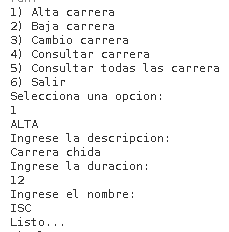
\includegraphics[width=\textwidth]{alta.png}
 \caption{Creamos un registro}
 \label{fig:alta}
\end{center}
\end{figure}

\subsection{Consulta}
\begin{figure}[H]
\begin{center}
 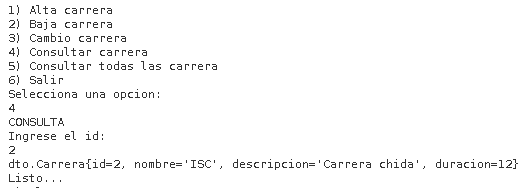
\includegraphics[width=\textwidth]{consulta.png}
 \caption{Consulta con base en un id}
 \label{fig:consulta}
\end{center}
\end{figure}

\subsection{Consultar todos}
\begin{figure}[H]
\begin{center}
 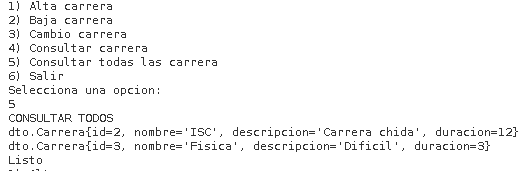
\includegraphics[width=\textwidth]{todos.png}
 \caption{Se consultan todos}
 \label{fig:todos}
\end{center}
\end{figure}

\subsection{Baja}
\begin{figure}[H]
\begin{center}
 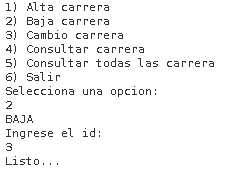
\includegraphics[width=\textwidth]{baja.png}
 \caption{Borramos un registro}
 \label{fig:baja}
\end{center}
\end{figure}

\subsection{Cambio}
\begin{figure}[H]
\begin{center}
 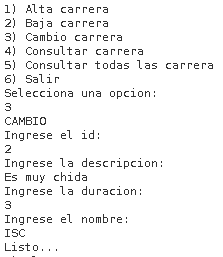
\includegraphics[width=\textwidth]{cambio.png}
 \caption{Realizamos cambios con base en un id}
 \label{fig:cambio}
\end{center}
\end{figure}

\begin{figure}[H]
\begin{center}
 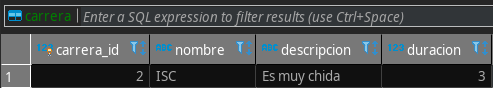
\includegraphics[width=\textwidth]{final.png}
 \caption{Registros de la base de datos después del cambio y la baja}
 \label{fig:final}
\end{center}
\end{figure}


\section{Conclusiones}
Este fue un pequeño ejemplo de como implementar el patrón DAO, con ello podemos 
utilizar el código de este ejercicio en futuras practicas y lo importante es 
que se entendió el como trabajar siguiendo dicho patrón y lo que este nos 
permite realizar.

\end{document}
